% !TEX encoding = UTF-8 Unicode
%!TEX root = ../Main/thesis.tex
% !TEX spellcheck = en-US
%%=========================================
\documentclass[../Main/thesis.tex]{subfiles}
\begin{document}
\chapter{Prototype Evaluation}
\label{ch:evaluation}

\section{Preparations}
\begin{figure}[h]
	\centering
	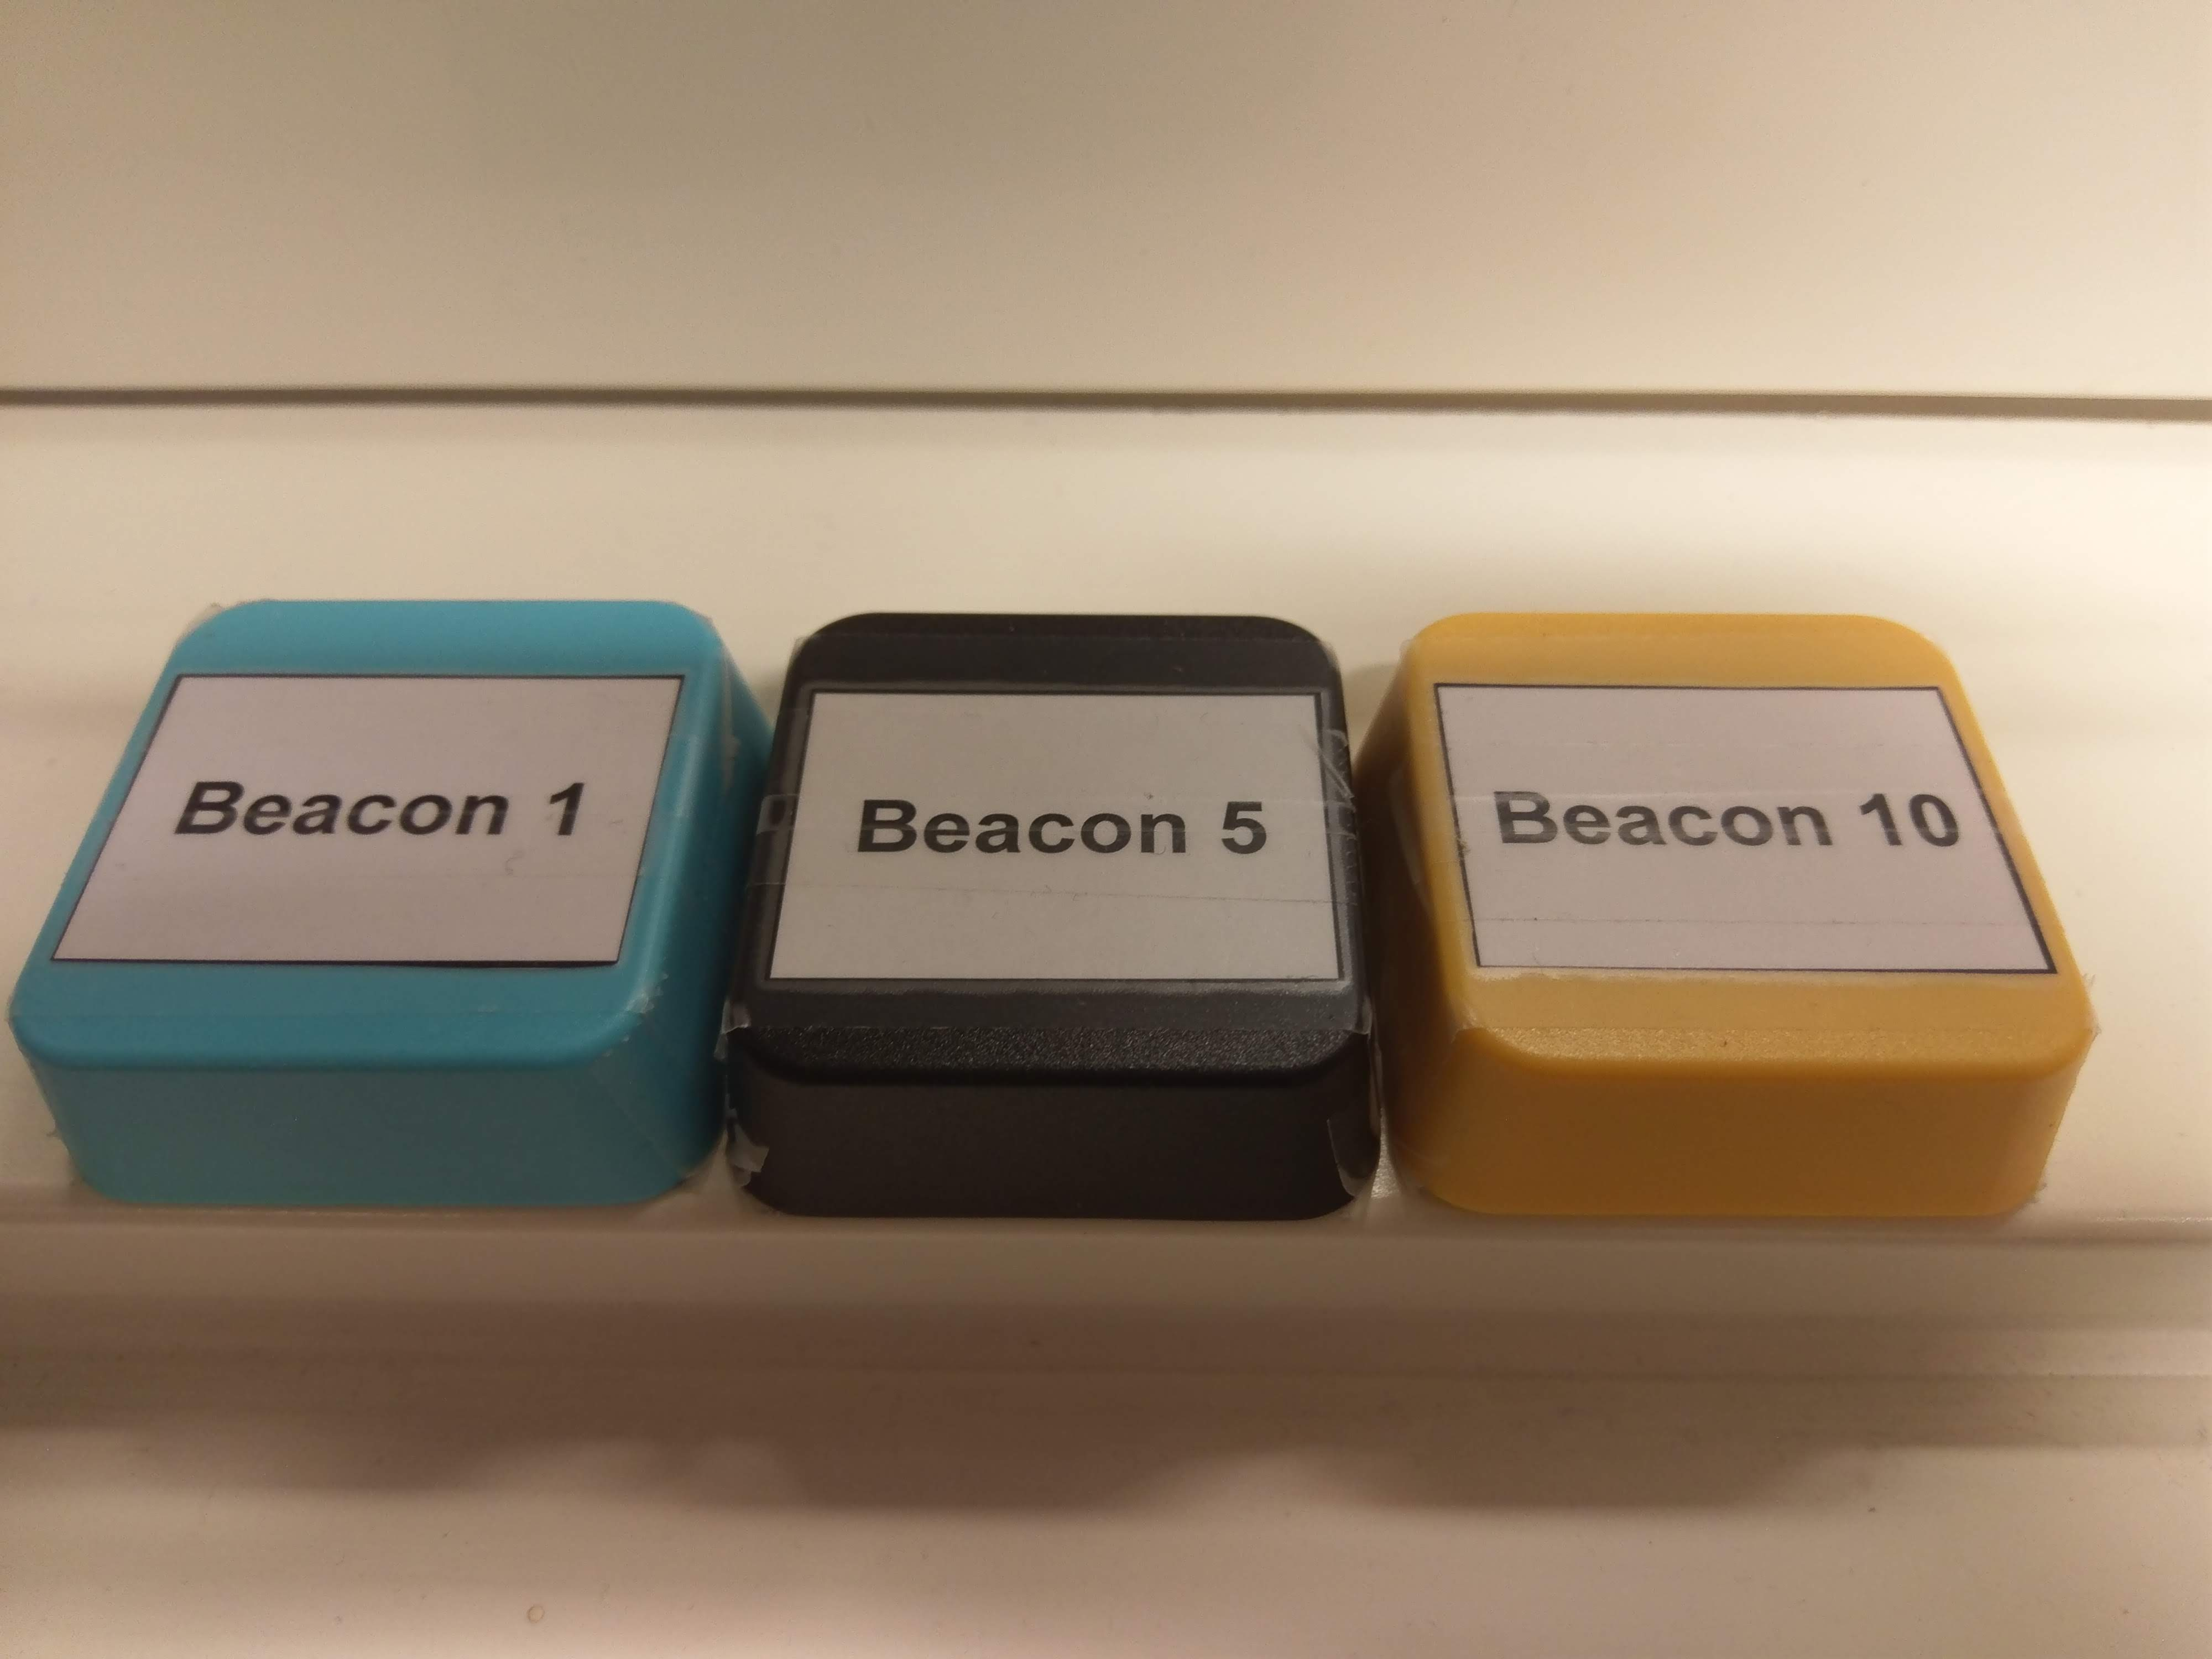
\includegraphics[width=\textwidth]{../fig/beacons}
	\caption{Numbered BLE beacons}
	\label{fig:beacons}
\end{figure}
\section{Test of FireTracker}

\begin{figure}[h]
	\centering
	\begin{subfigure}{0.45\textwidth}
		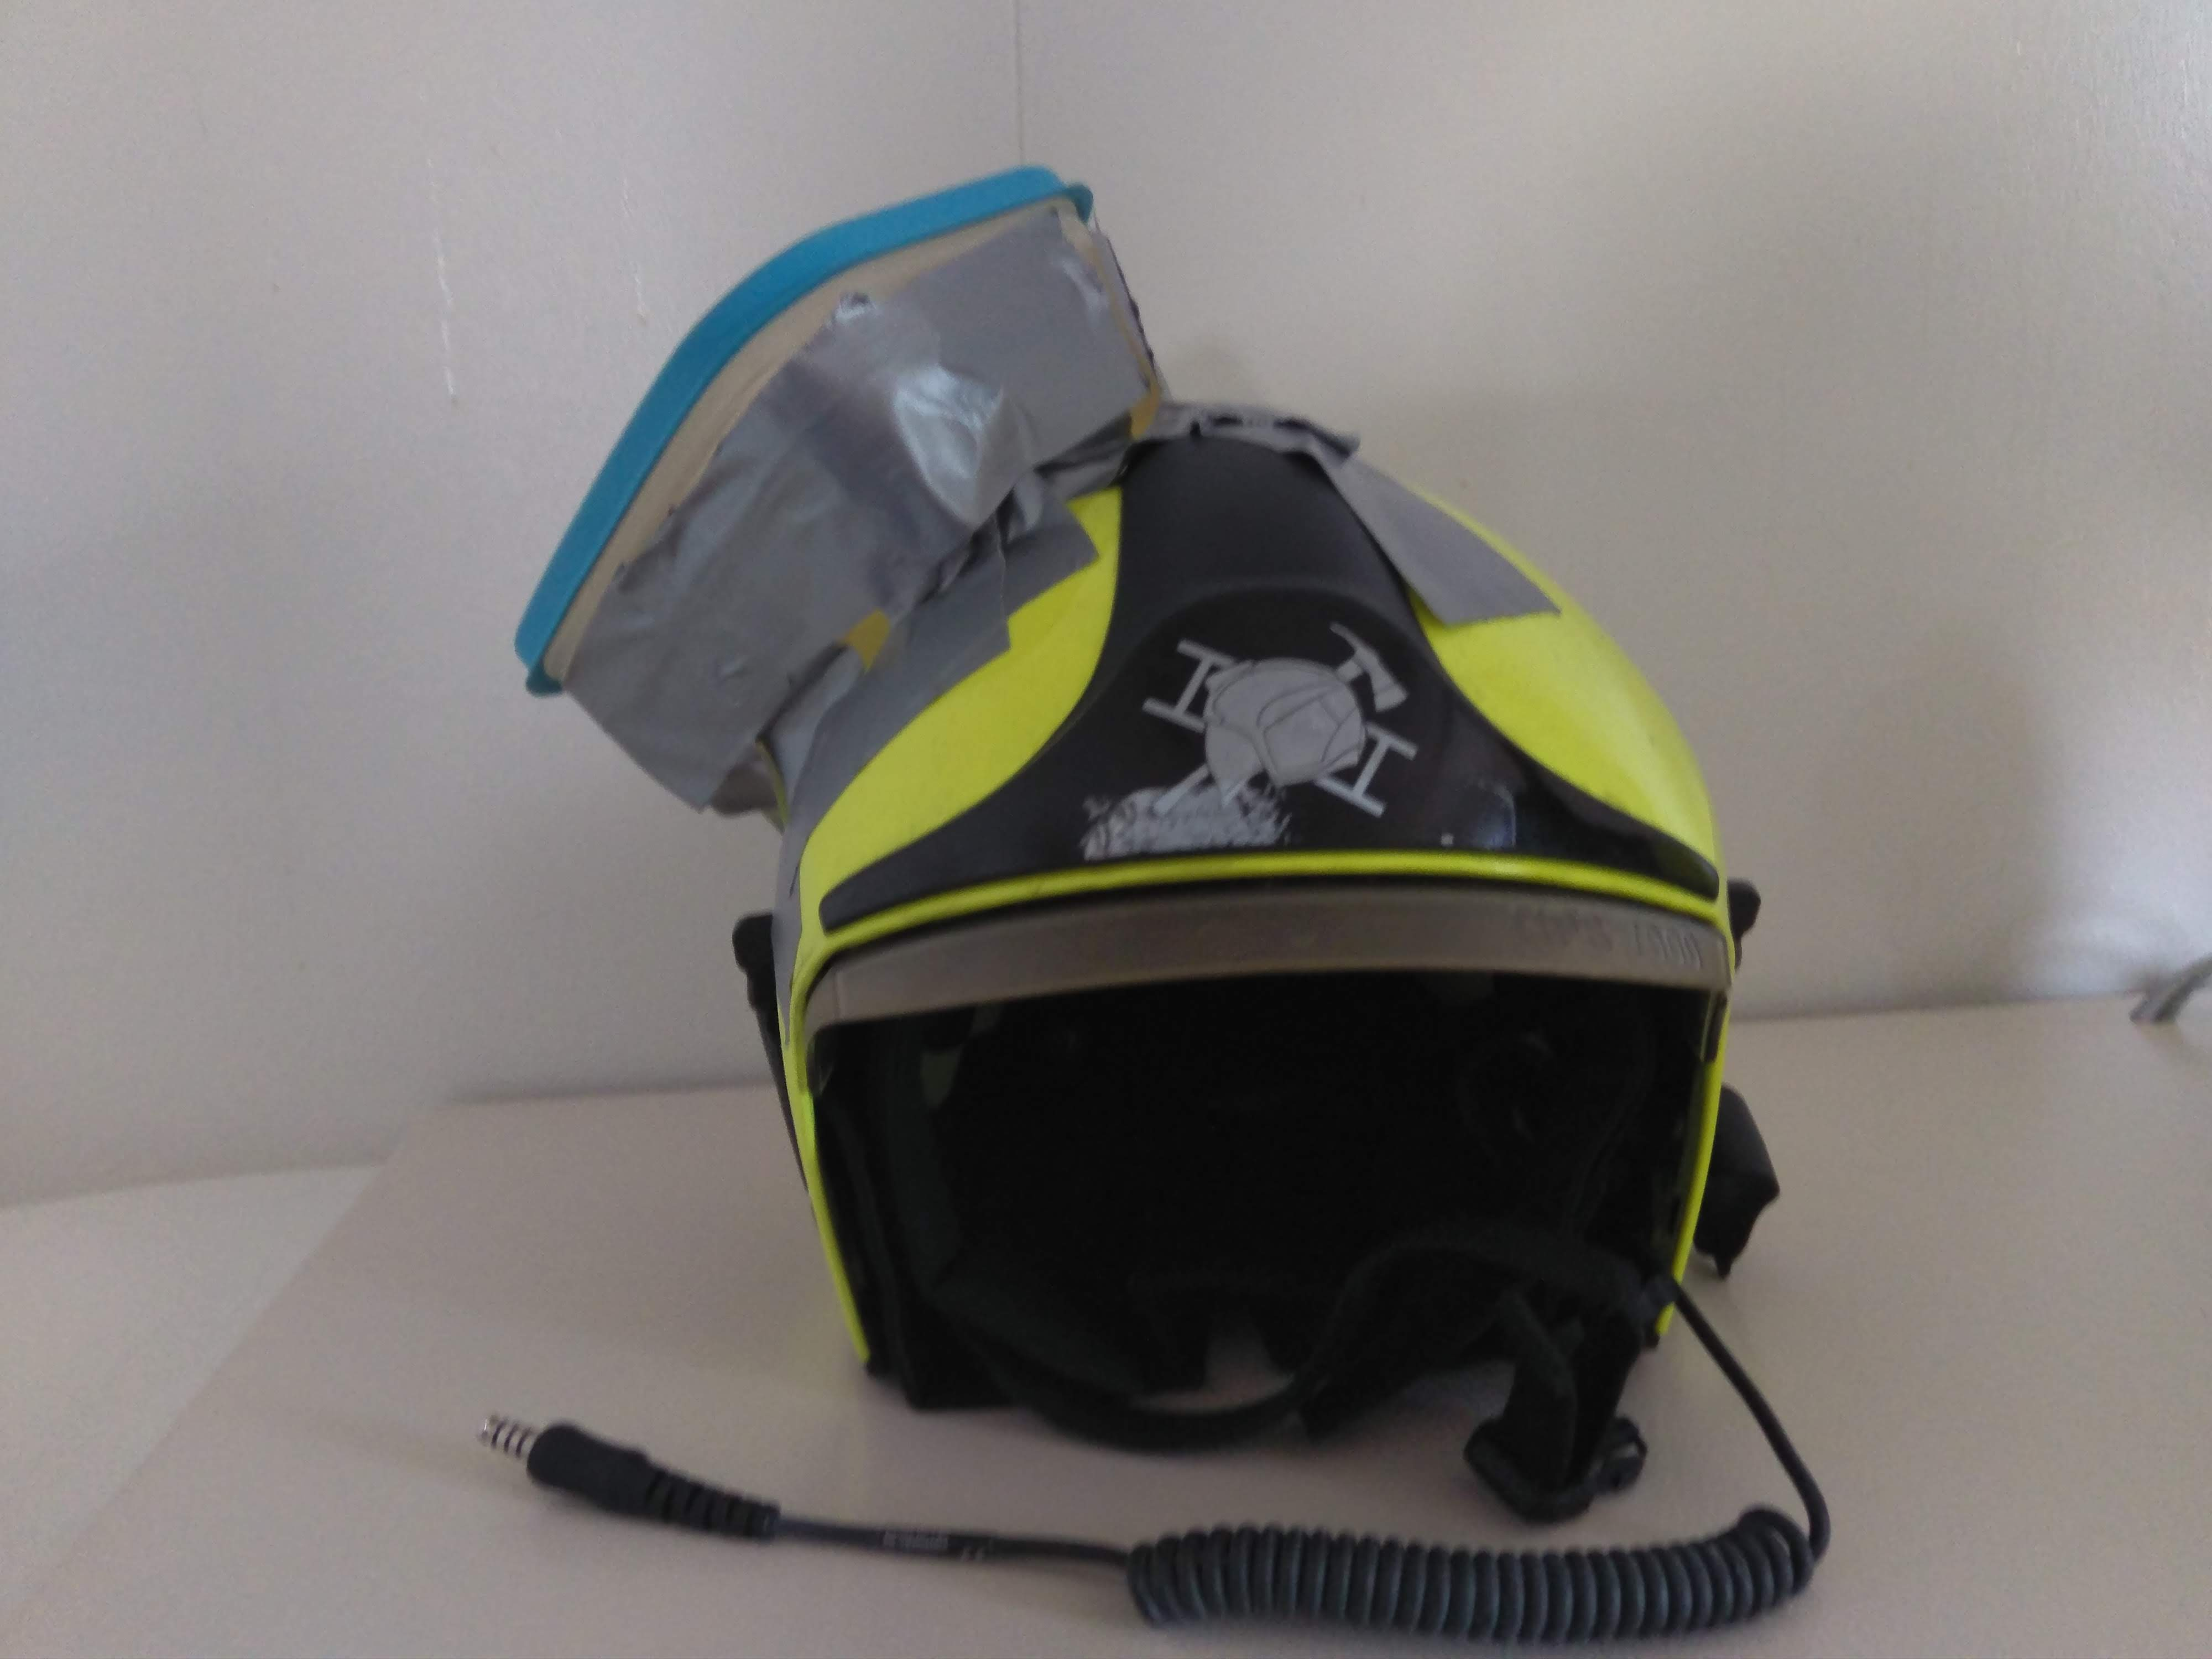
\includegraphics[width=\textwidth]{../fig/helmet-front}
		\caption{Front of helmet}
		\label{fig:eval-helmet-front}
	\end{subfigure}
	\begin{subfigure}{0.45\textwidth}
		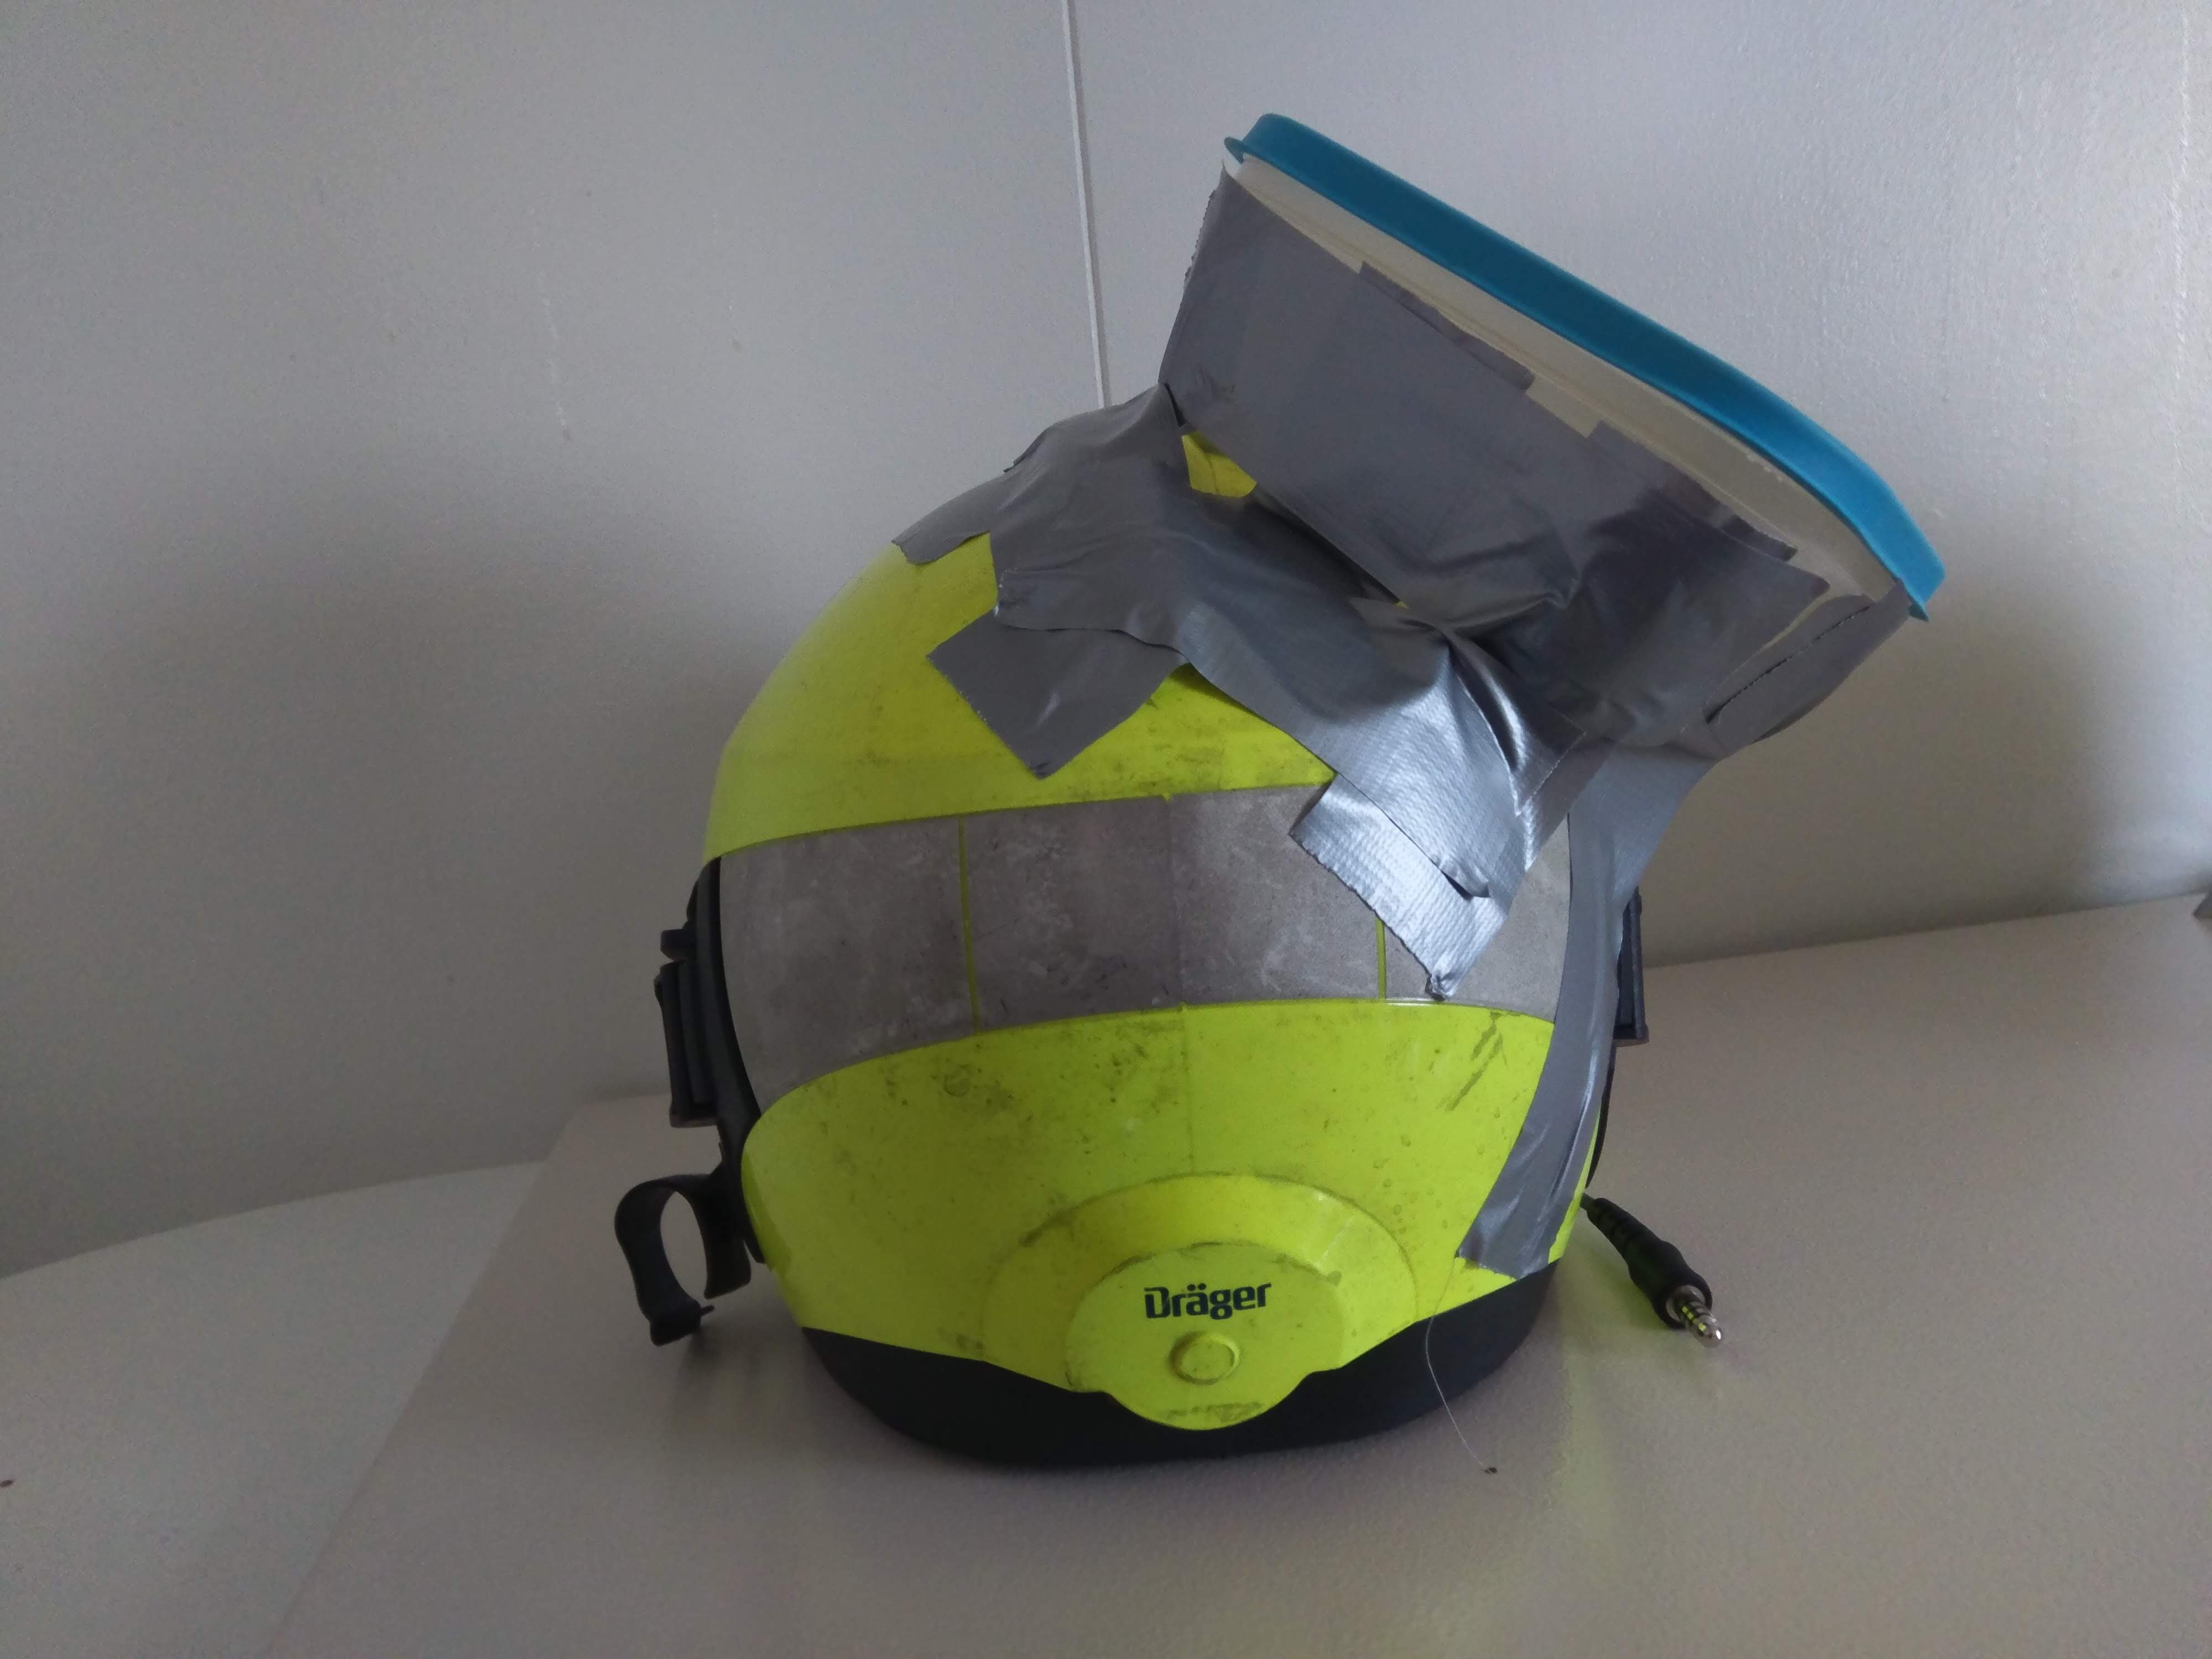
\includegraphics[width=\textwidth]{../fig/helmet-back}
		\caption{Backside of helmet}
		\label{fig:eval-helmet-back}
	\end{subfigure}
	\begin{subfigure}{0.45\textwidth}
		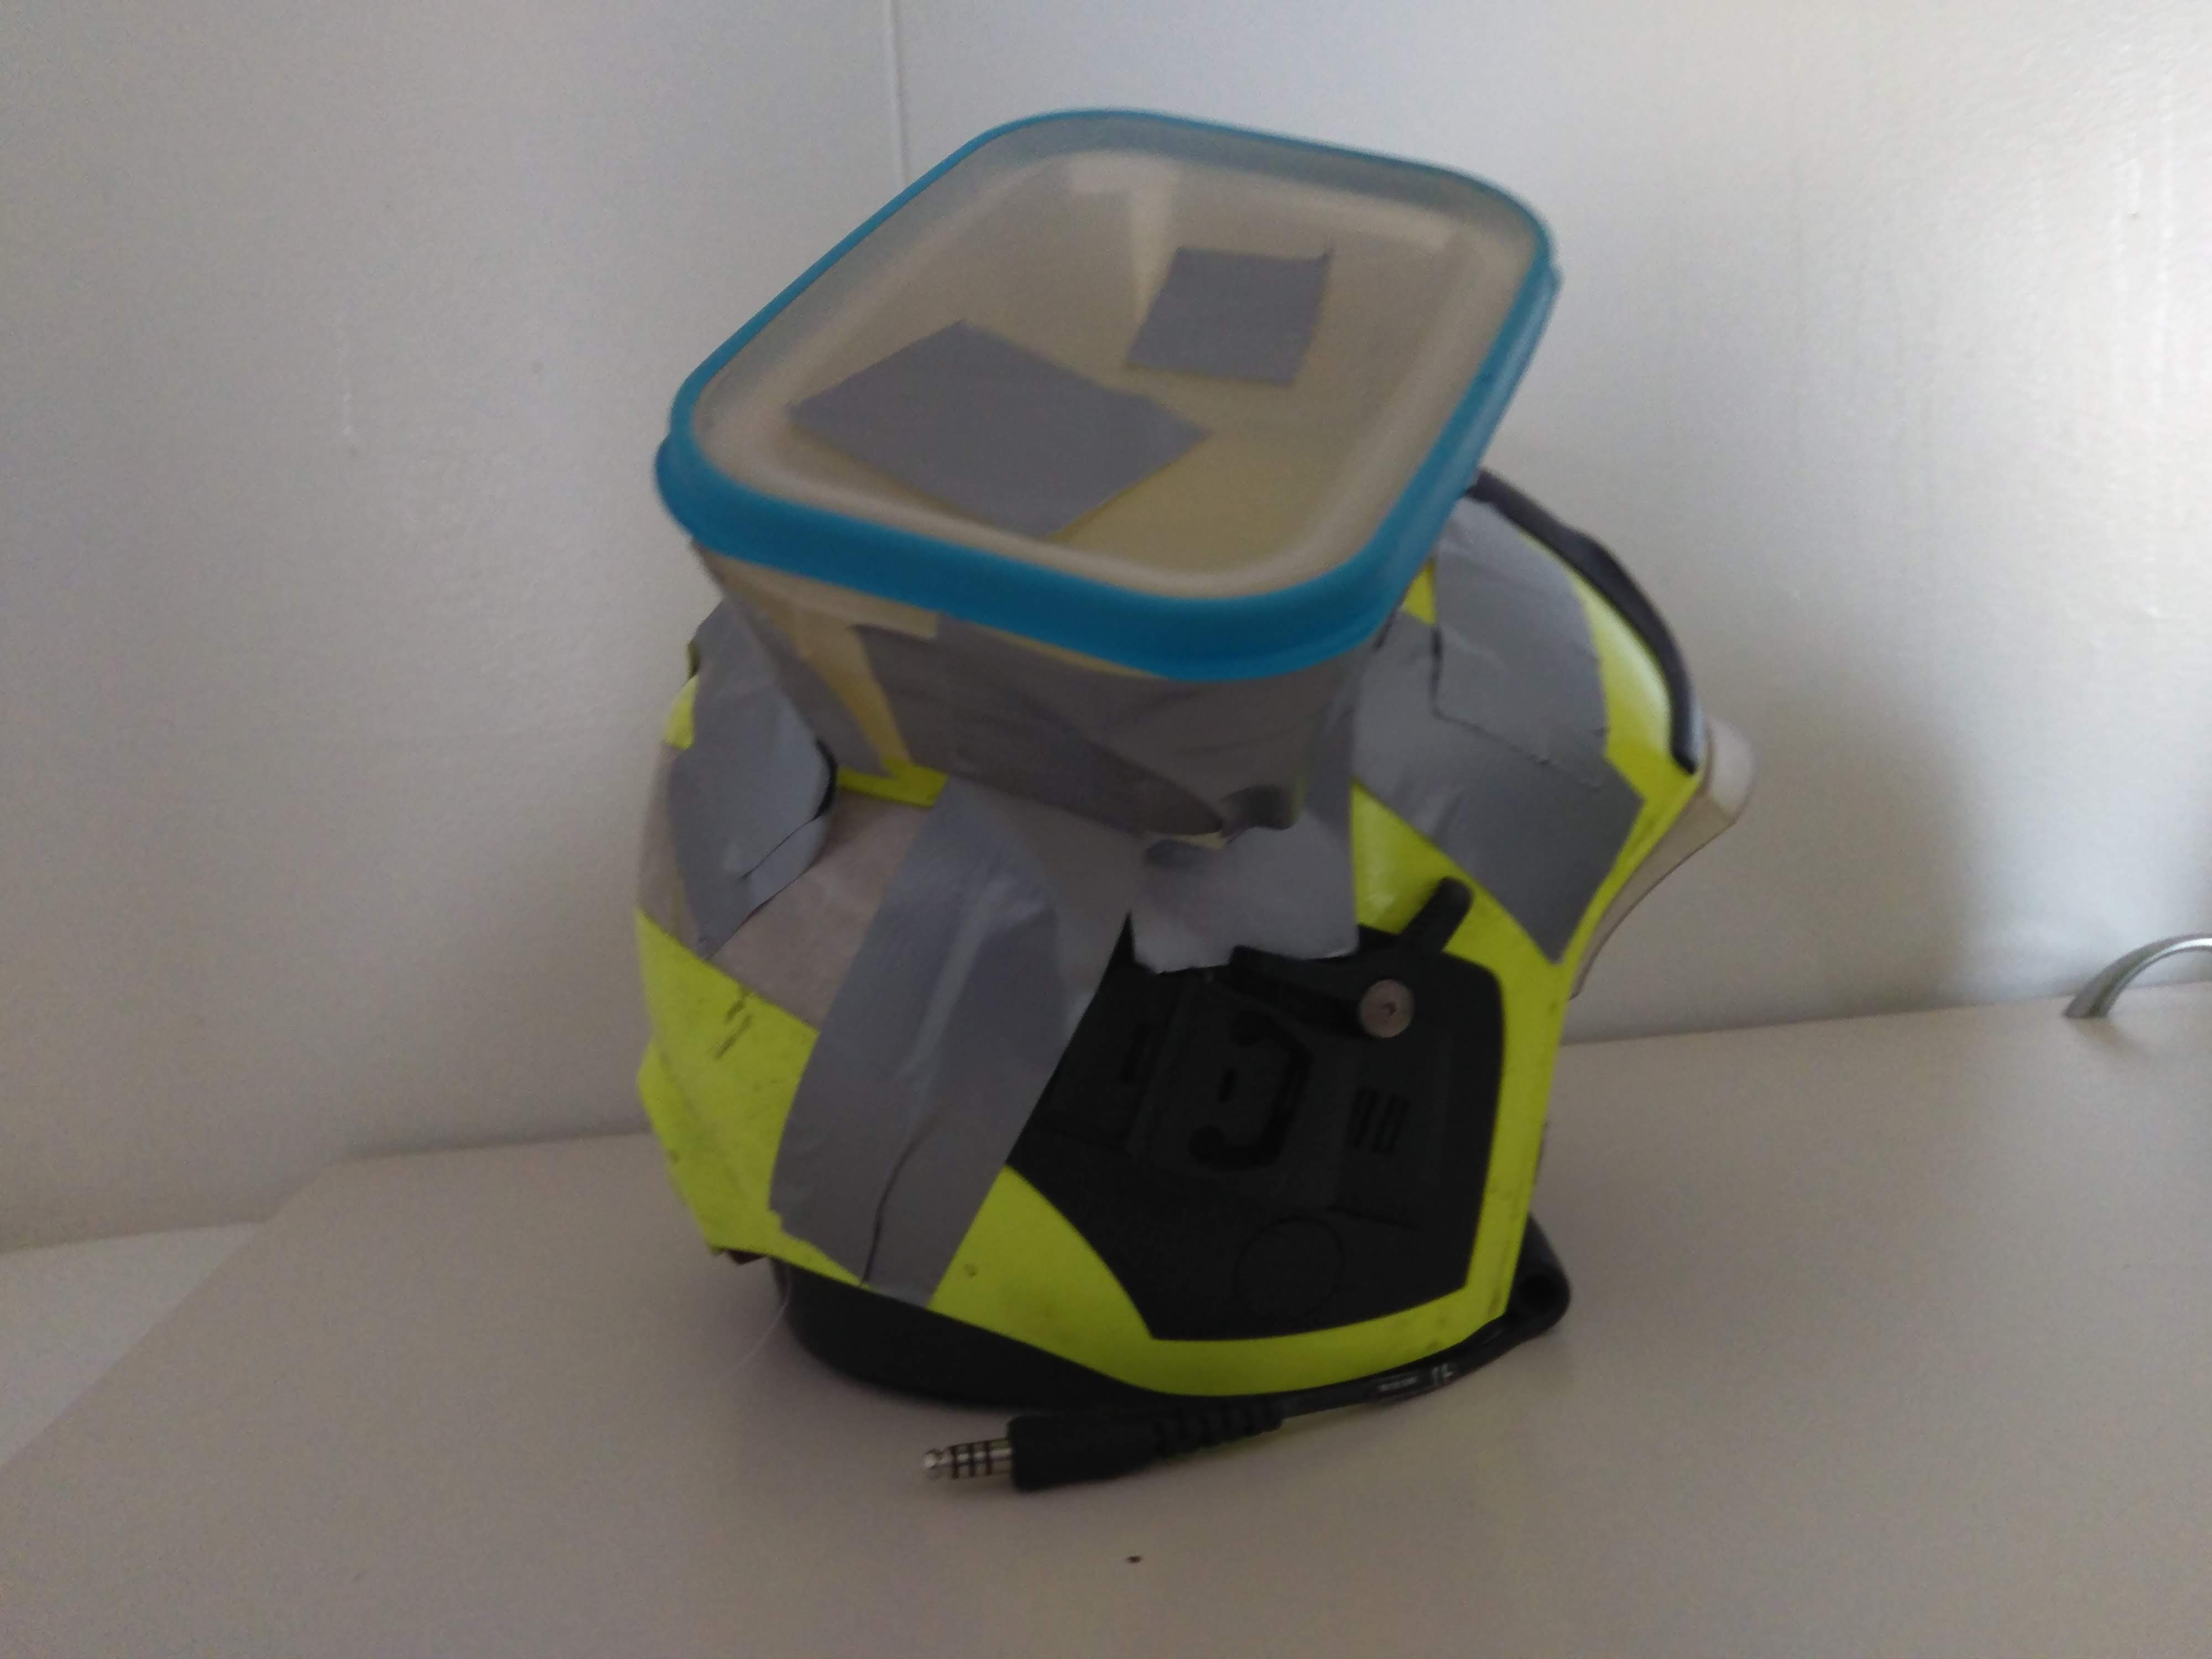
\includegraphics[width=\textwidth]{../fig/helmet-right}
		\caption{Right side of helmet}
		\label{fig:eval-helmet-right}
	\end{subfigure}
	\begin{subfigure}{0.45\textwidth}
		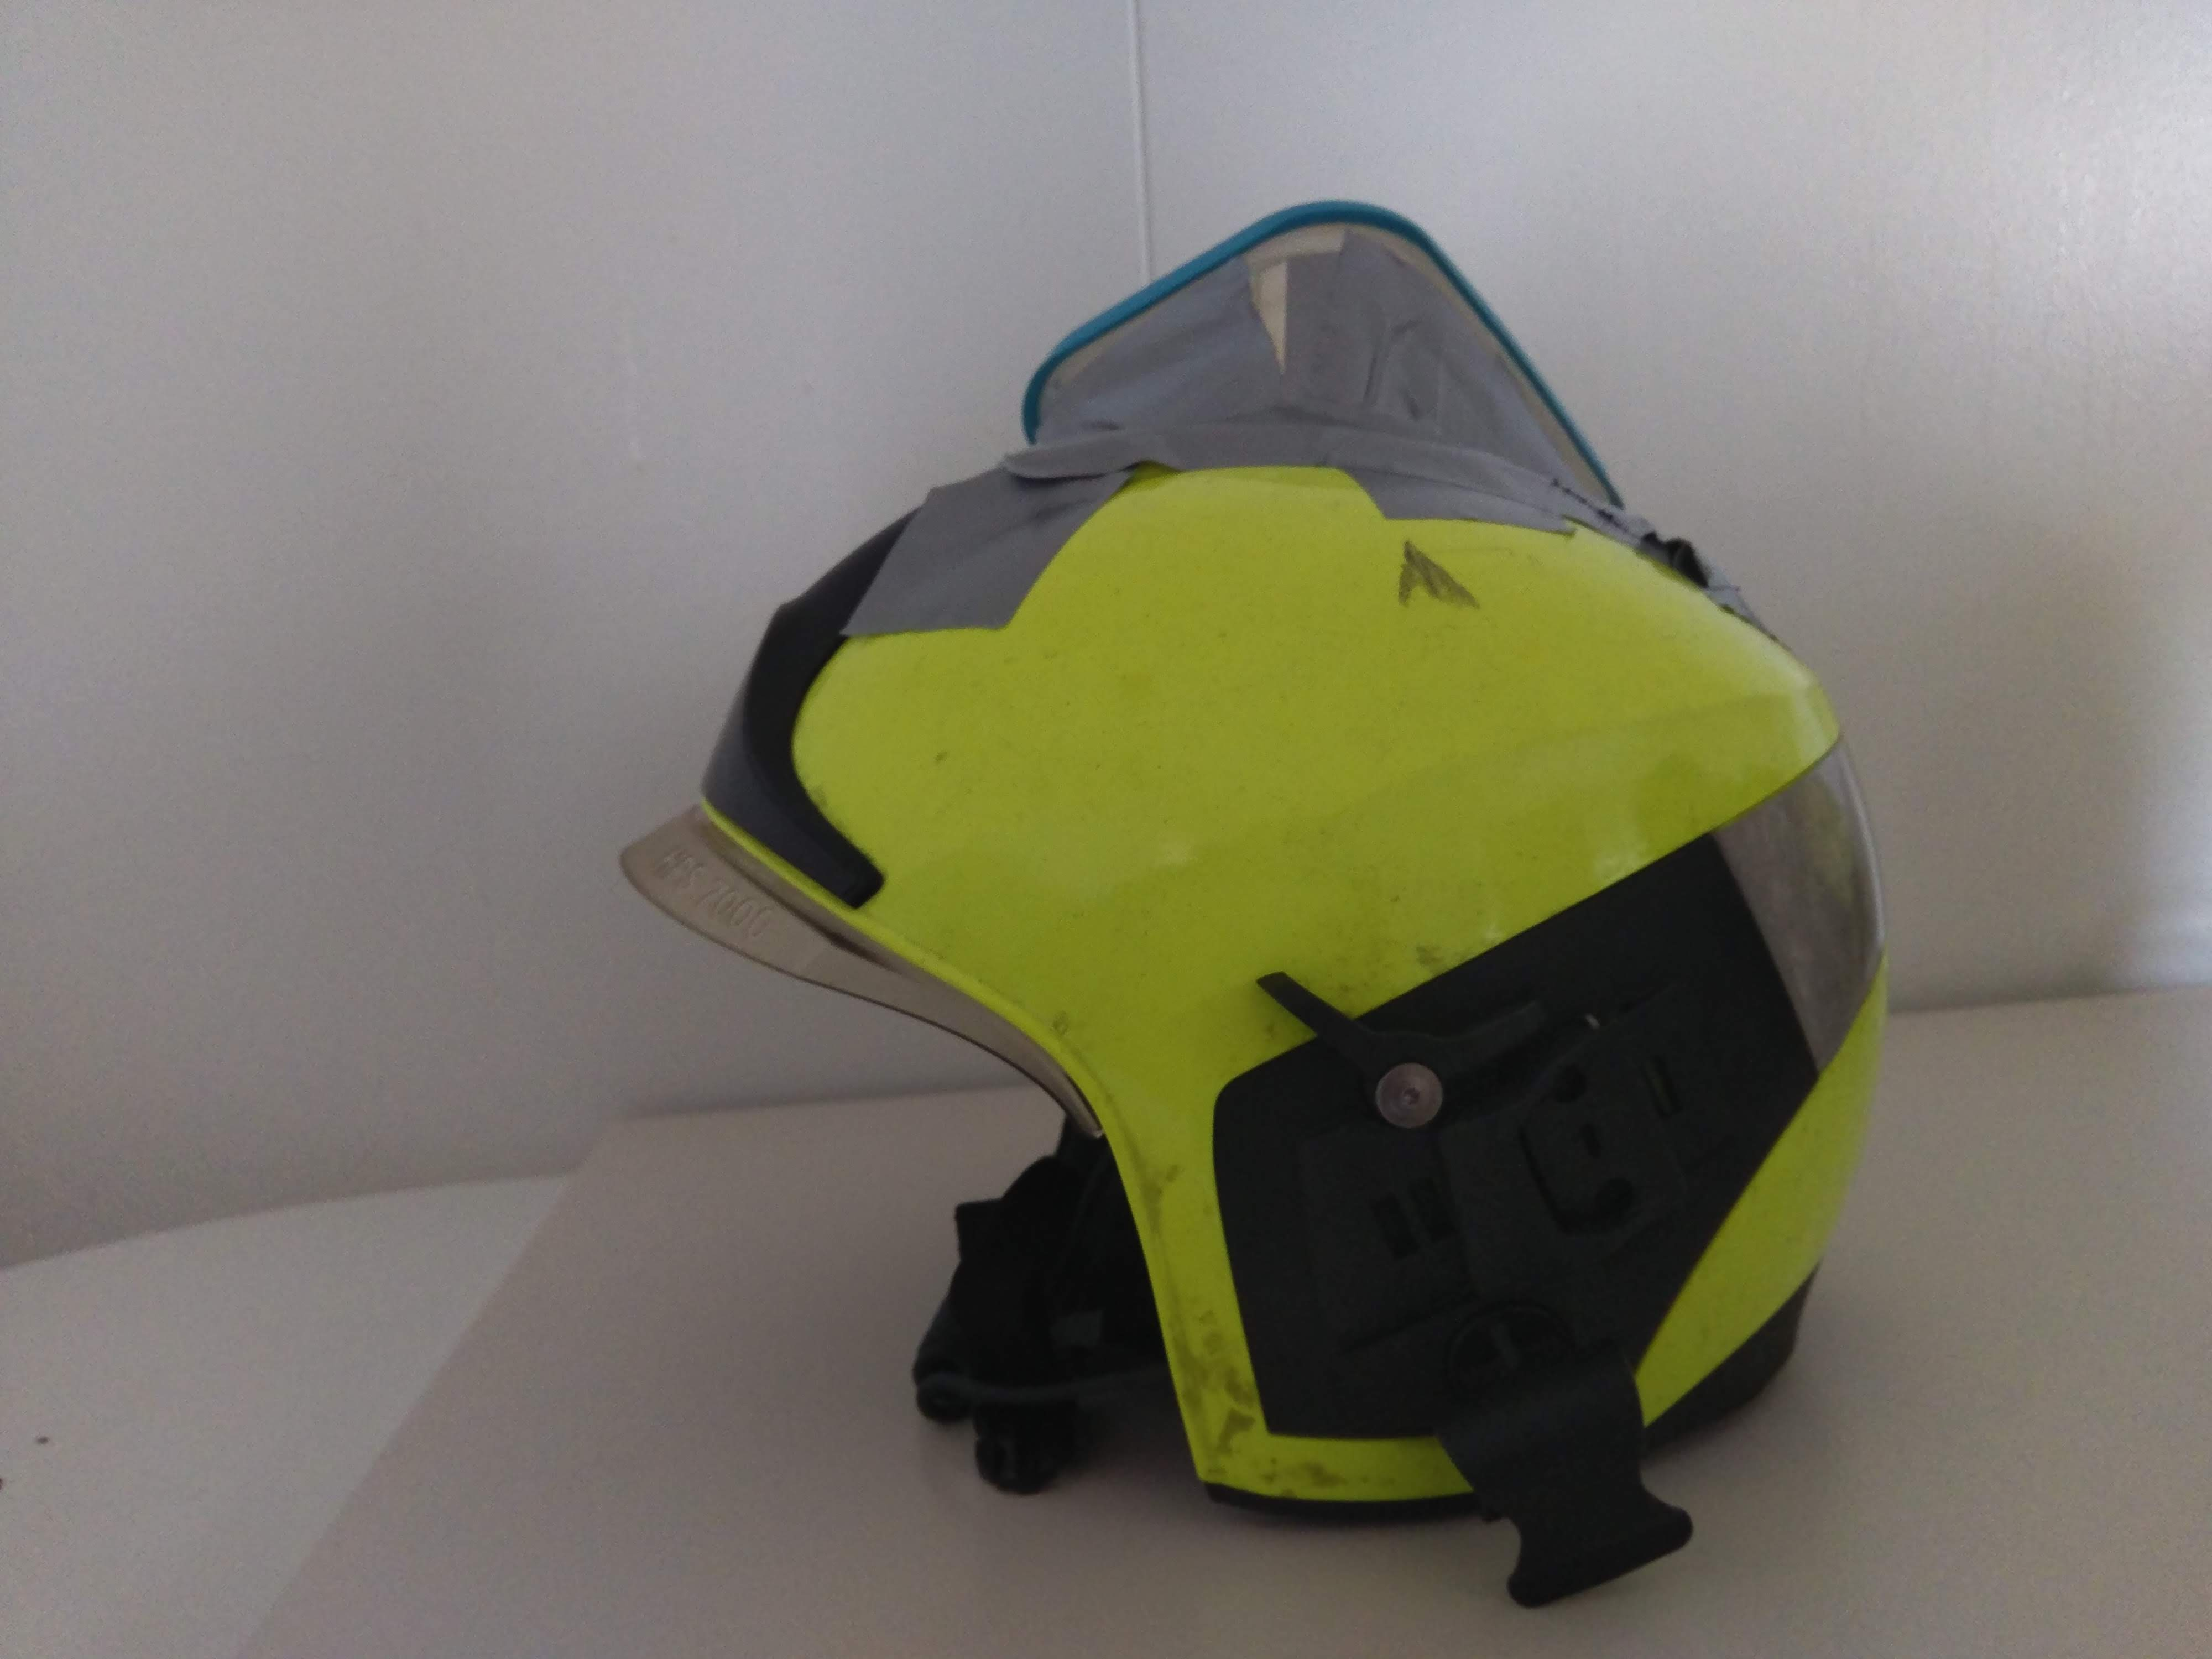
\includegraphics[width=\textwidth]{../fig/helmet-left}
		\caption{Left side of helmet}
		\label{fig:eval-helmet-left}
	\end{subfigure}
	\caption{Plastic box for smartphone attached to helmet}
	\label{fig:eval-helmet}
\end{figure}

\begin{figure}[h]
	\centering
	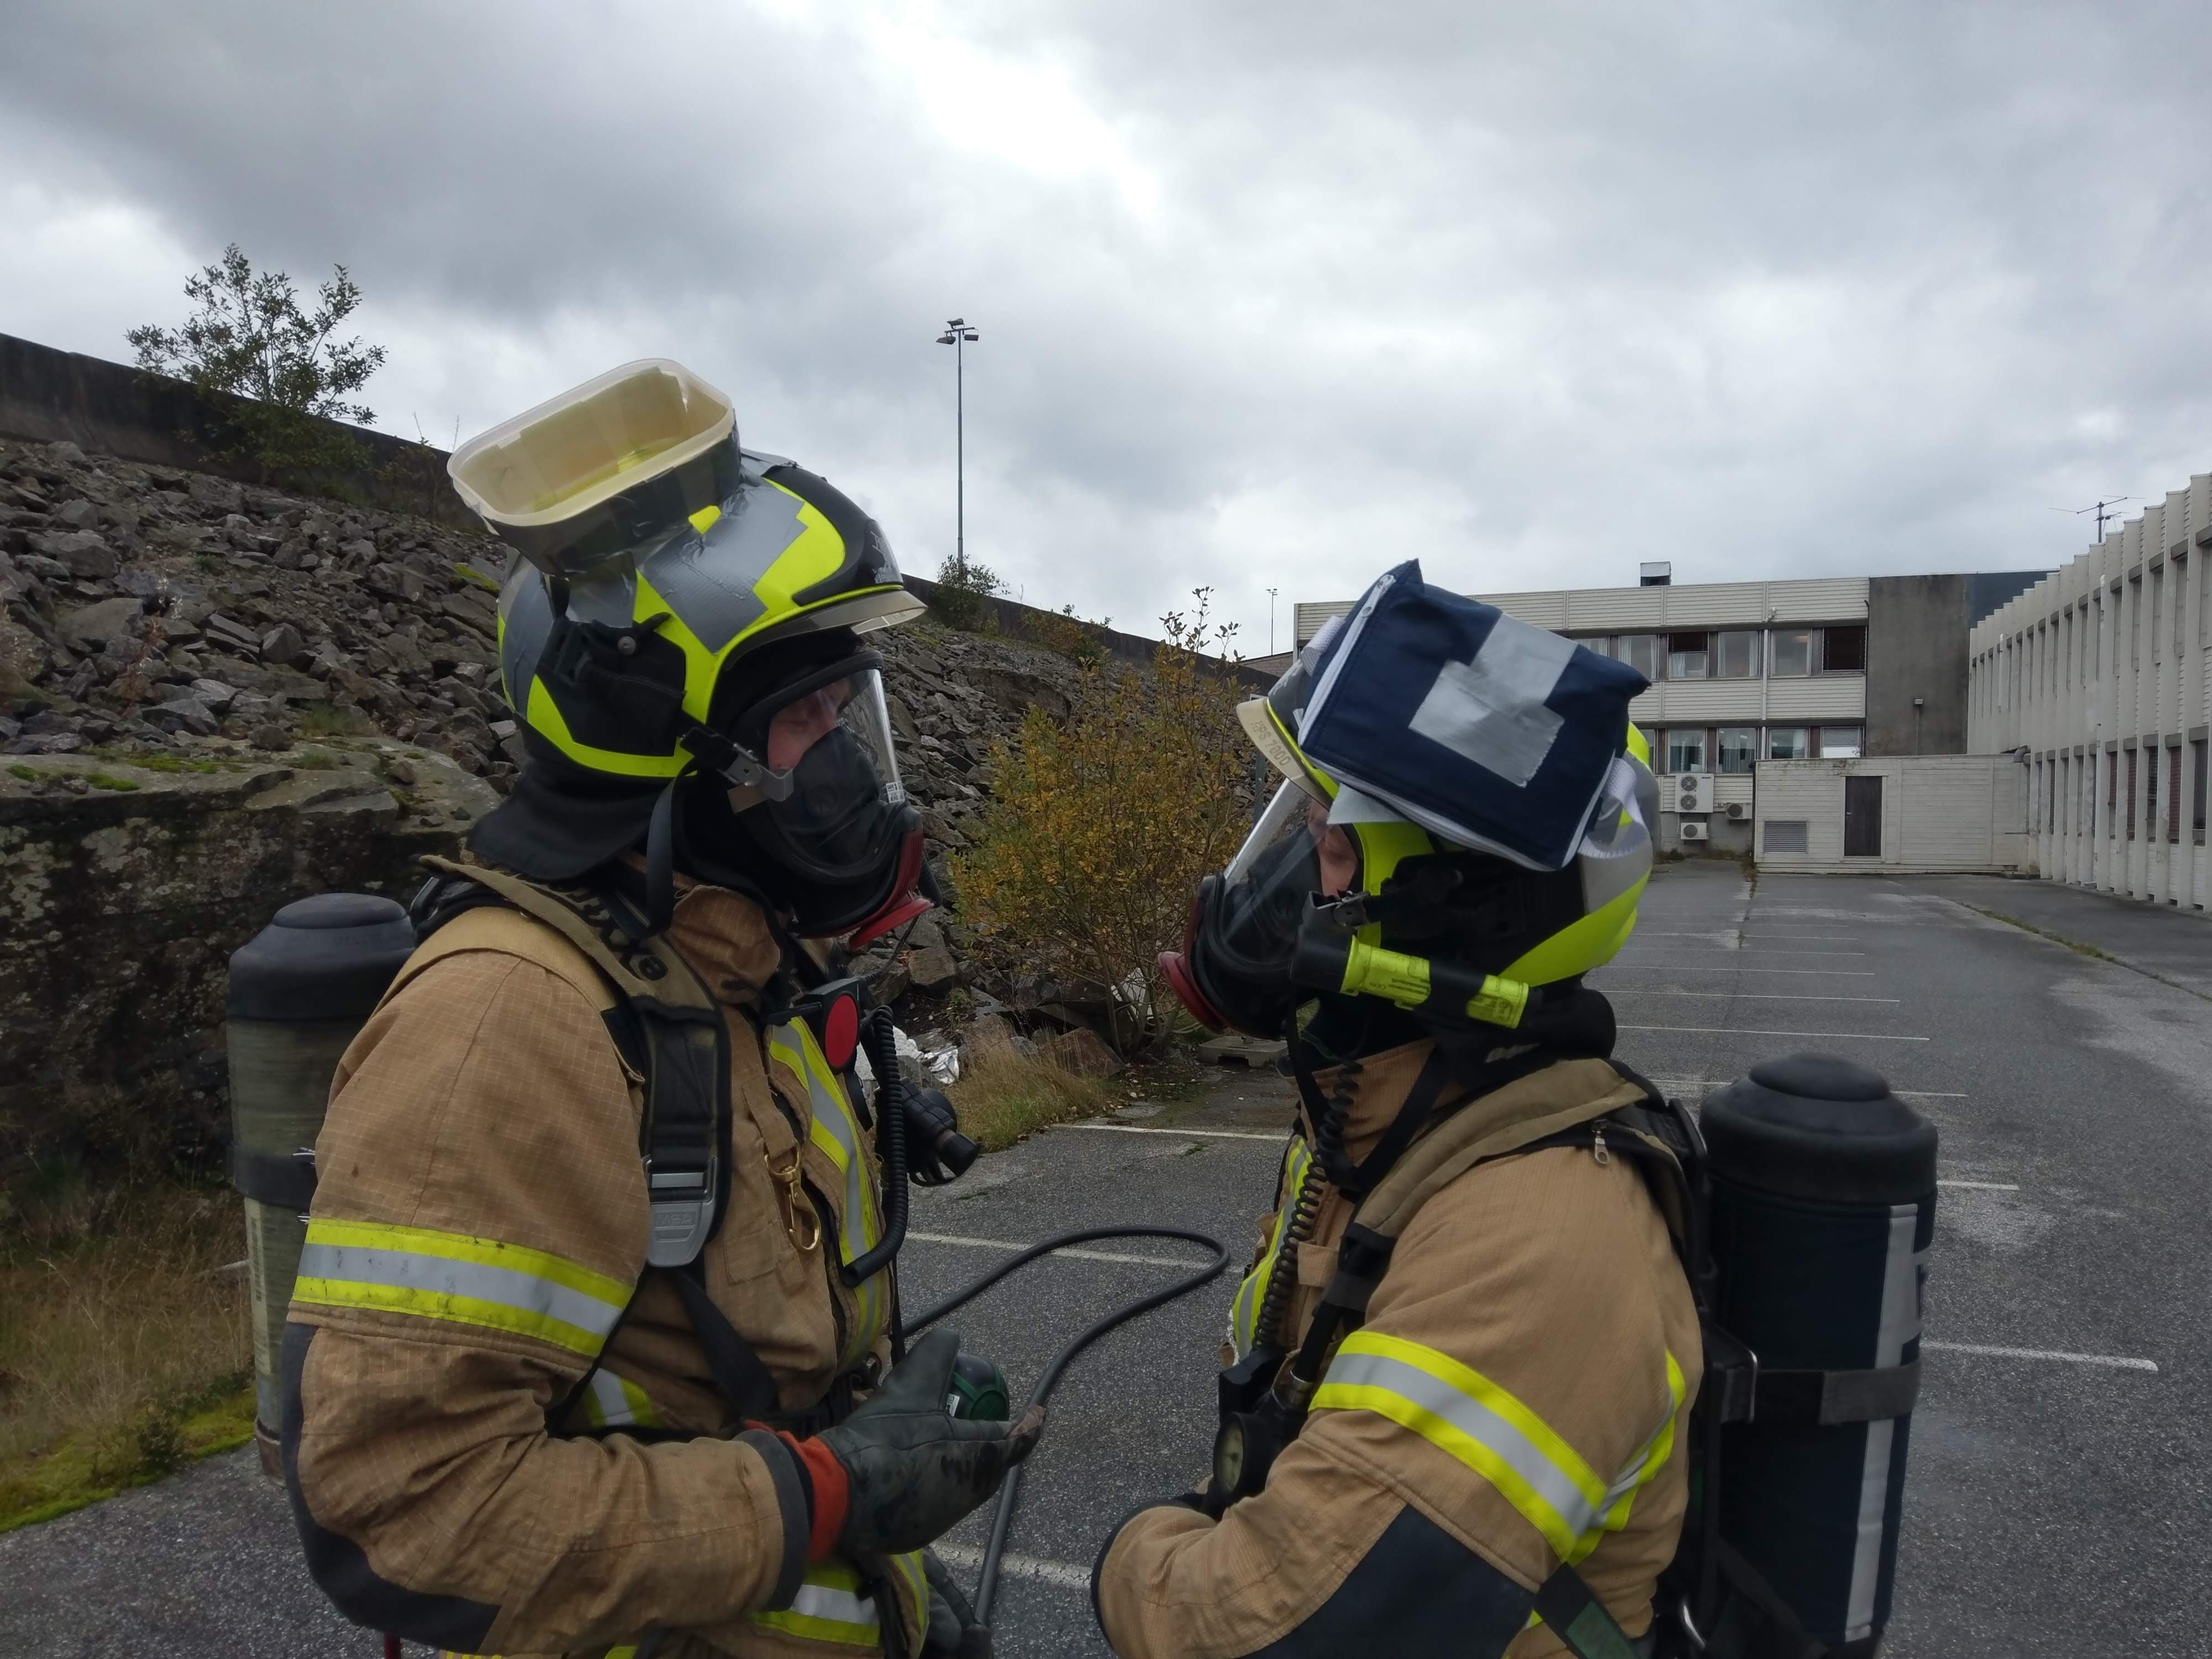
\includegraphics[width=\textwidth]{../fig/firefighters-with-helmet}
	\caption{Firefighters with smartphones mounted on their helmet}
	\label{fig:eval-firefighters}
\end{figure}

\section{Interview}

\section{System Usability Scale}

\end{document}
